\documentclass{article}
\usepackage{graphicx}
\usepackage{hyperref}
\usepackage{url}

\setlength{\parskip}{1em}

\begin{document}

 
\title{Editing Geometries}

This article is designed to outline the basic controls of ICE's Geometry Editor.

\section{Getting Started}

Once ICE is installed on your computer, there are no further dependencies or
preparation required to use the Geometry Editor.

\section{Opening a Geometry Editor}

To open a Geometry Editor in ICE, you have three options:

\begin{center}
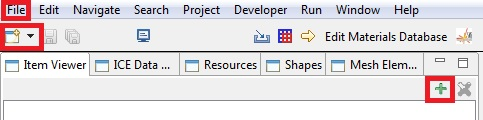
\includegraphics[width=12cm]{images/CreateNewGeometryOptions.jpg}
\end{center}

Top to bottom, they are:

1) Click the File menu, then New, then Other\ldots and select the Create Item
Wizard in the new dialog and press Next. Then, select Geometry Editor from the
list and press Finish.

 
2) Click the New button. Select Create Item Wizard in the new dialog and
press Next. Then, select Geometry Editor from the list and press Finish.


3) Enter the ICE Perspective by clicking the Open Perspective button in the
upper right corner of the screen, select ICE from the dialog that pops up, and
click OK. Afterwards, click the Create an Item button, select Geometry Editor,
and click OK.

\section{Working with the Geometry Editor}

\section{Camera}

You can change the perspecive of the camera by clicking and dragging inside the
Geometry Editor. You can see this initially by the way the three axes and the
reference plane move as you rotate the camera about the origin. Scrolling the
mouse wheel will zoom the camera in or out.

\section{Primitive Shapes}

\begin{center}
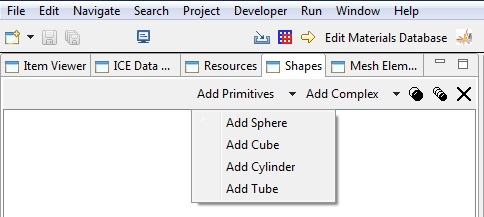
\includegraphics[width=12cm]{images/GeometryAddPrimitive.jpg}
\end{center}

Simple shapes can be added with the Add Primitives dropdown menu in the Shapes
view. Simply select an object from the menu to add it to the scene.

\begin{center}
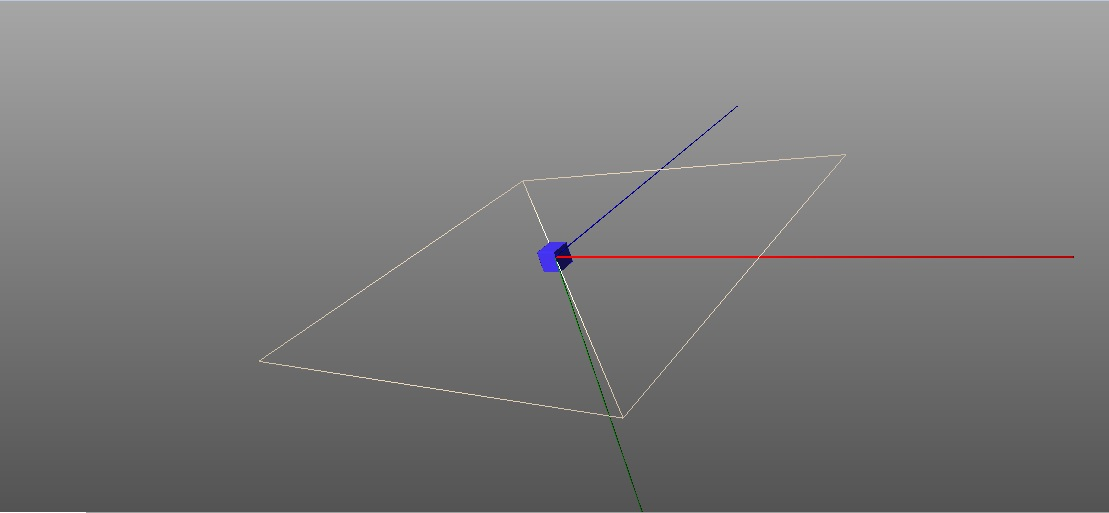
\includegraphics[width=12cm]{images/GeometryAddCube.jpg}
\end{center}

Clicking on the shape's name in the Shapes View will cause that shape to turn
red in the editor.

\begin{center}
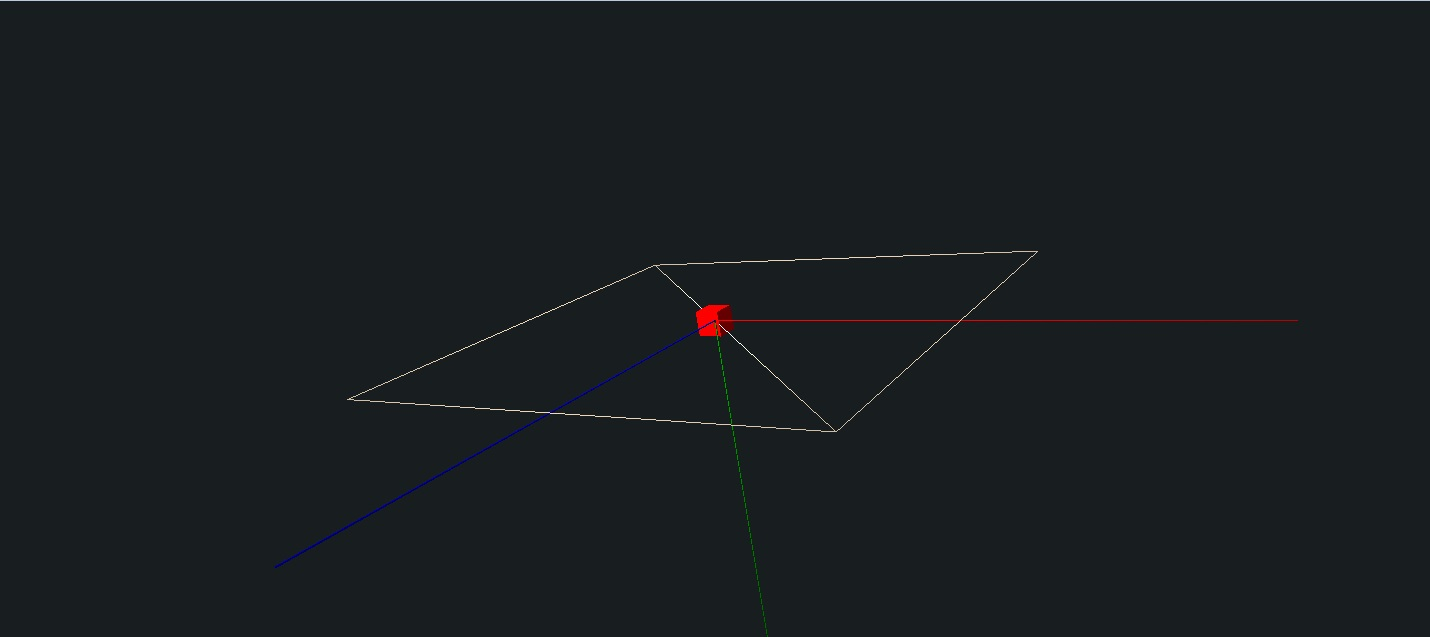
\includegraphics[width=12cm]{images/GeometrySelectCube.jpg}
\end{center}

Selections in the Shapes View also activate the Transformation View in the lower
left corner. Editing the values in this view will change the selected shape
accordingly.

\begin{center}
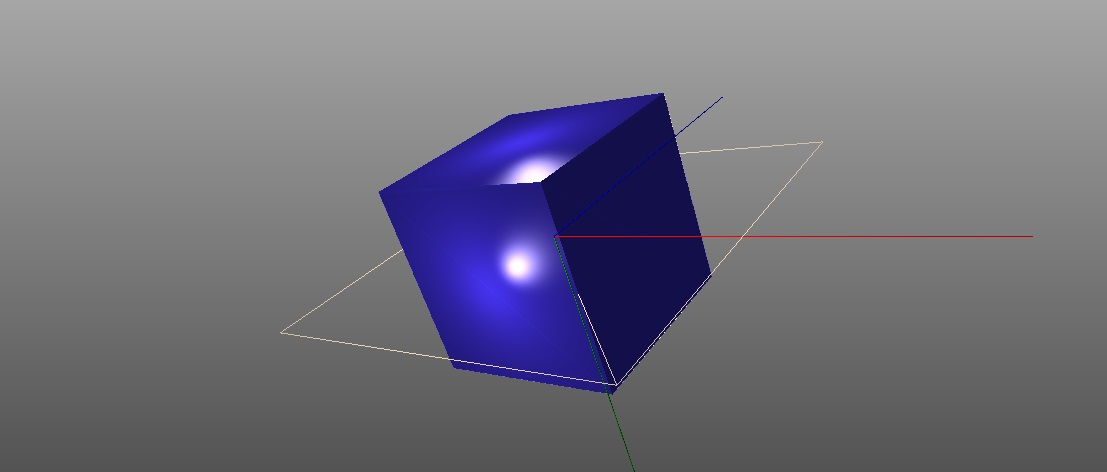
\includegraphics[width=12cm]{images/GeometryCubeSize.jpg}
\end{center}

\textbf{Size} - Controls the overall size of the shape. Setting size to X is
equivalent to setting the shape's three scales to X times their current value.

\begin{center}
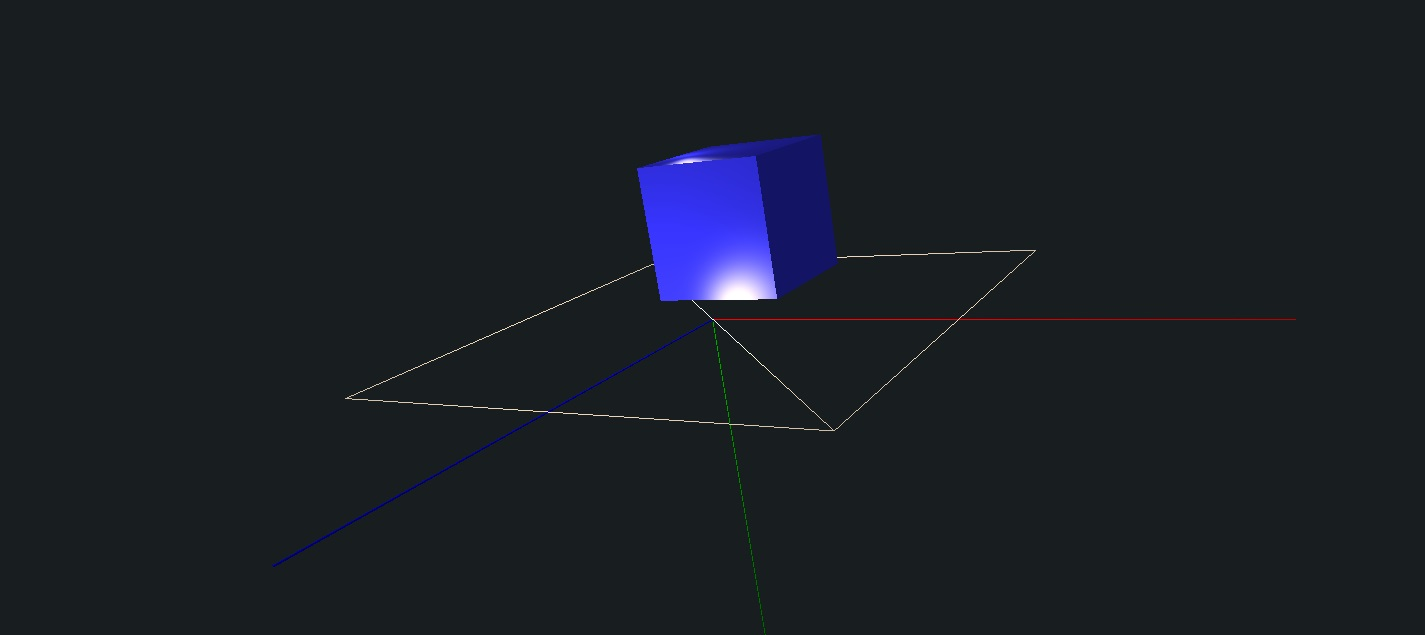
\includegraphics[width=12cm]{images/GeometryCubeTranslate.jpg}
\end{center}

\textbf{Translate} - Controls the position of the shape. Setting one of the
translations will move the shape that many units along the given axis.

\begin{center}
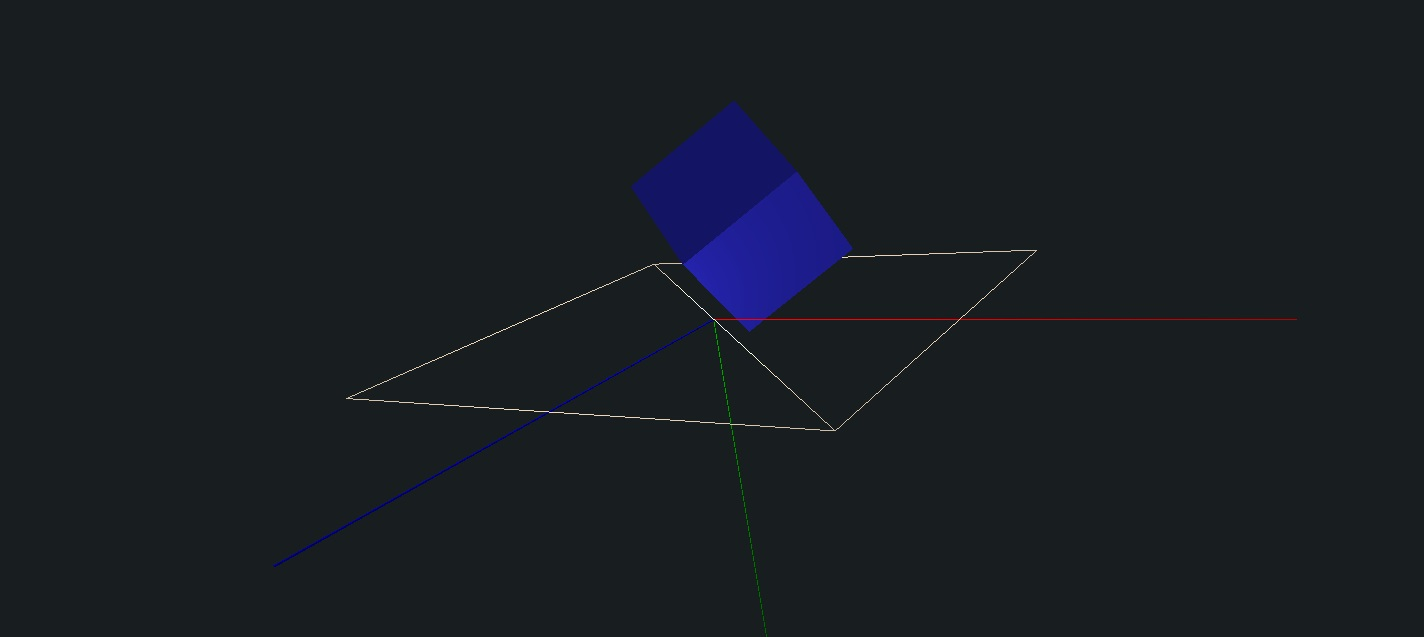
\includegraphics[width=12cm]{images/GeometryCubeRotate.jpg}
\end{center}

\textbf{Rotation} - Controls the orientation of the shape. Setting one of the
rotations will rotate the shape the given number of degrees about that axis.

\begin{center}
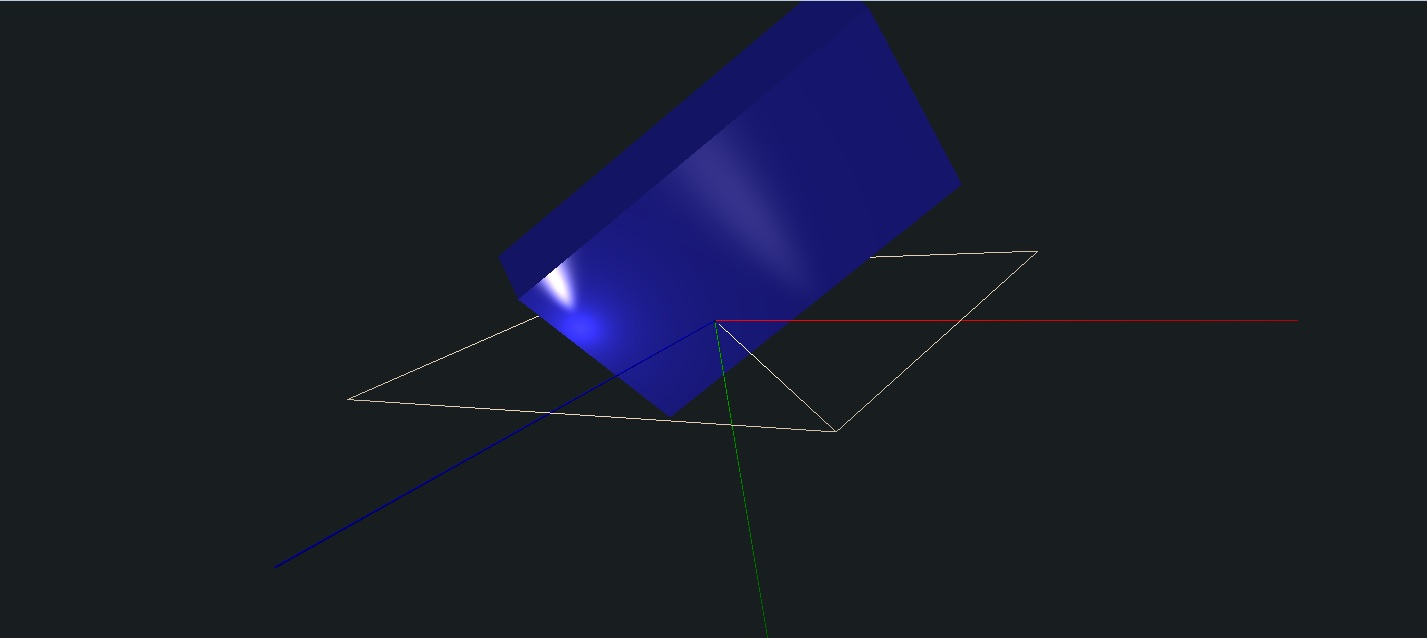
\includegraphics[width=12cm]{images/GeometryCubeScale.jpg}
\end{center}

\textbf{Scale} - Controls the size of the shape in three directions. Setting one
of the scales will stretch or compress the shape in that direction by a factor
of the scale's new setting.

\section{Complex Shapes}

Multiple primitive shapes can be combined within a single grouping for easier
editing. First, create a complex shape using the Add Complex button. 

\begin{center}
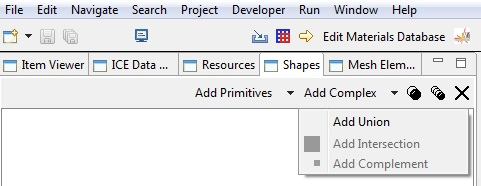
\includegraphics[width=12cm]{images/GeometryAddComplex.jpg}
\end{center}

Currently, only unions are supported. The union will appear in the Shapes View
with an empty spot for a child shape. 

\begin{center}
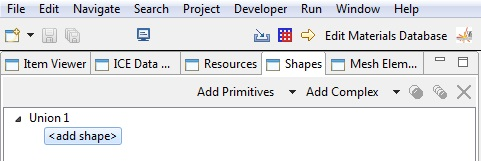
\includegraphics[width=12cm]{images/GeometryUnionAddShape.jpg}
\end{center}

Select \textless Add Shape\textgreater and add a primitive shape as before to
add the shape as a child of the union. To add additional shapes, select the
child shape and add another as normal.

Selecting the union will select all of its child shapes, and changes to the
transformation view will affect the entire complex shape. Individual shapes can
still be selected for editing on their own.

You can add a complex shape as a child to a complex shape in the same way as a
primitive shape, allowing for nested unions

\begin{center}
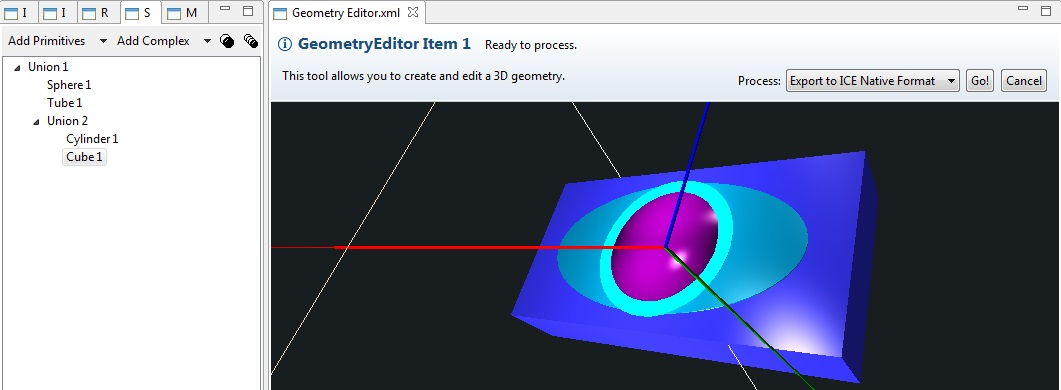
\includegraphics[width=12cm]{images/GeometryStackedUnions.jpg}
\end{center}

\section{Copying}

Once you have a shape created, you can automatically create copies of that
shape. 

\begin{center}
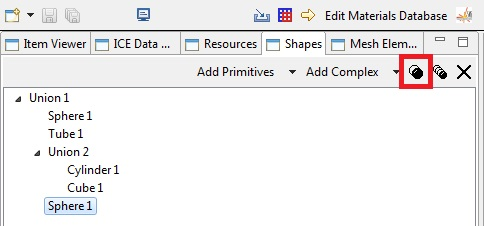
\includegraphics[width=12cm]{images/GeometryDuplicateShape.jpg}
\end{center}

Press the Duplicate Shape button, highlighted above, to create an exact copy of
the selected primitive shape. The copy will appear as the child of the same
complex shape as the original, if any, and can be modified independently after
creation.

\begin{center}
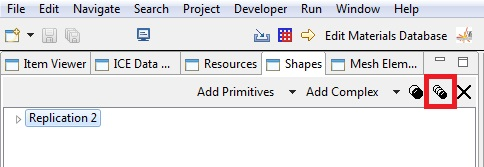
\includegraphics[width=12cm]{images/GeometryReplicateShape.jpg}
\end{center}

You can systematically create many copies of a shape with the Replicate Shape
button highlighted above. This will open a new dialog.

\begin{center}
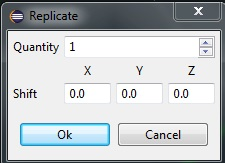
\includegraphics[width=12cm]{images/GeometryReplicateDialog.jpg}
\end{center}

The quantity is the number of desired copies of the shape which should be in the
replication. This includes the orignal (ie setting quantity to 2 will result in
2 shapes, the original and a copy).

The Shift boxes allow you to specify an offset to be placed between each copy.
For example, if you set X to 100 and Y to 50, then each copy will be 100 units
along the X axis and 50 along the Y away from the previous copy. 

The original shape and all copies will be placed in a new complex shape, which
will take the original shape's position in the tree.

\section{Deletion}

You may remove a shape and all its children by selecting it in the Shapes view
and clicking the Delete button, highlighted below.

\begin{center}
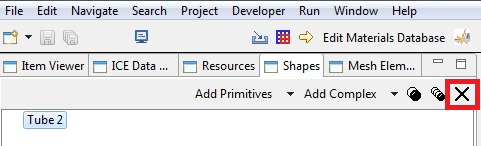
\includegraphics[width=12cm]{images/GeometryDeleteButton.jpg}
\end{center}

\end{document}
